\documentclass[twocolumn]{article}
\usepackage[margin=0.7in]{geometry}

\usepackage[small,compact]{titlesec}

\usepackage{graphicx}
\usepackage{listings}
\usepackage{color}
\usepackage{hyperref}


\title{COMP 6360 Wireless and Mobile Networks \\ Project 2 Report}
\author{Team 2\thanks{Jiao Yu [jzy0012], Song Gao [szg0031], Xinyu Que [xzq0003] (ordered by first name)}}
\date{April, 2012}

\begin{document}

\maketitle

\section{Architecture}
\par{The simulator consists of four threads and multiple classes. As shown in Figure~\ref{fig:arch}, they work collaboratively to simulate the OLSR Protocol and EEBL application. Section~\ref{sec:design} discusses details of each part of the system.}
\begin{figure}[htb]
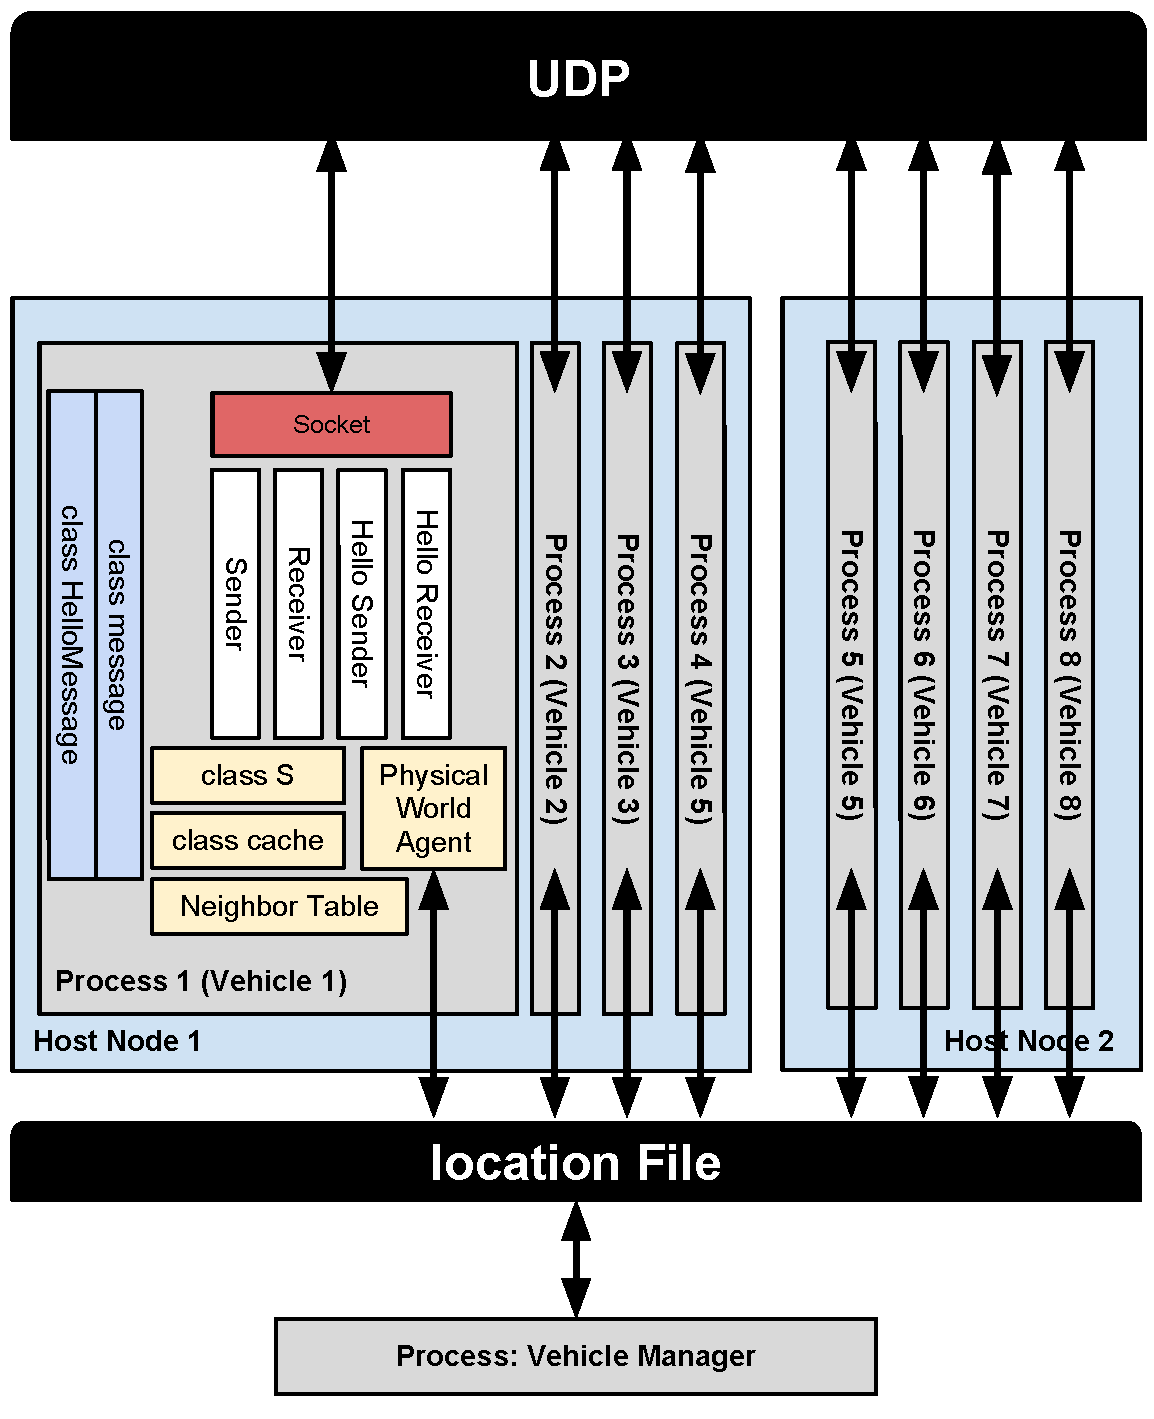
\includegraphics[width=\columnwidth]{fig/arch.pdf}
\caption{Architecture}
\label{fig:arch}
\end{figure}

\section{Design}
\label{sec:design}
\par{A lot of modules implemented in our project 1 are reused, including the message modeling and serialization, fast cache for EEBL and beacon messages, configuration class, etc.. Several new modules are designed and implemented for the sake of:
    \begin{enumerate}
    \item Using OLSR's MPR concept for rebroadcasting decisions;
    \item Implementing dynamic traffic, i.e., the vehicles are mobile.
        \end{enumerate}
    This section describes in detail design of new modules introduced in project 2.}
    \subsection{OLSR building blocks}
{\bf Involved classes: } {\tt Neighbor Table, MPR selectors Table, Hello Message}
\par{{\tt Neighbor Table} class is in charge of managing neighbors and computing MPRs. It has three main responsibilities:}
\subsubsection{constructing neighbor table from Hello Messages}
\par{The Neighbor Table class constructs a table from Hello messages, which stores all the 1 hop neighbors and also neighbors of them. We use C++ std::map as the data structure to hold this table. Table~\ref{tab:data} shows an example of neighbor table for Node 1.}
\begin{table}[htb]
\begin{center}
\begin{tabular}{|r|c|r|c|r|c|}
\hline  
{\bf 1 hop neighbors}      & {\bf neighbors of it}     \\ \hline
2    &                     1, 3, 4, 8        \\ \hline
5    &                     1, 4, 6, 7          \\ \hline
8    &                     1, 2     \\ \hline
\end{tabular}
\caption{An example of neighbor table}
\label{tab:data}
\end{center}
\end{table}
\par{When a new Hello message is received, Neighbor Table class checks whether the originator of the message is already in neighbor table or not. If it is, neighbors of the originator and also timestamp for this entry is updated. Otherwise a new entry is added.}
\subsubsection{Remove old entries}
\par{In addition to carrying data, {\tt Neighbor Table} class is also in charge of removing entries older than 3s, since previous neighbors may already moved away and no more Hello messages will be received from them. In order to do this, there is a timestamp associated with every entry in the table, in every 1s the update() method of this class is invoked which will remove old entries.}
\subsubsection{Compute MPRs}
\par{The algorithm to select MPRs should try to cover all 2 hop neighbors while minimizing the number of MPRs. We come up with an algorithm: First select the node which covers the maximum number of 2 hop neighbors as an MPR, then subtract the 2 hop neighbors covered by it from the entire set of 2 hop neighbors, repeat this step until the remaining 2 hop set is empty. This method may not be optimal, but it serves well for our purpose.}
\subsection{MPR selectors Table}

\par{The MPR selectors Table stores data about which nodes select me (the current node) as an MPR, so the current node will know whether to rebroadcast an eebl message by looking up this table. The data structure for this table is easy, it just needs to store a vector of node IDs and also their associated timestamp. By receiving an Hello Message, the MPR selectors class check the link status indicated by this Hello message. If it is MPR, then add the originator of it to that vector if the originator was not already there, otherwise update its timestamp. This class has a similar update() method as in Neighbor Table class, which will remove entries older than 3s.}
\subsection{Hello Message}

\par{Hello Message class has three fields: Originator ID, link status, and neighbors. In order to avoid variable length of packet size, which will complicate socket transmission of Hello Messages, we give the "neighbors" field fixed size of 120 bytes, which will hold up to 30 neighobrs ID. Usually a vehicle will have less than 30 one hop neighbors, the unused space of the 120 bytes are filled with unsigned int::MAX to indicate the end of this field.  
}
\par{The construction of a hello message should be based on neighbor table and the receiver node. From neighbor table we are able to extract the current node's one hop neighbors and MPRs. After putting originator ID and neighbors data into a hello message, the link status should be set properly according to whether the receiver node is one of the current node's MPRs. 
}

\subsection{Threads Implementation}
\par{We split the program into 4 threads, }
\begin{lstlisting}[language=C++,keywordstyle=\color{blue}]
    void * sender_main(void * context)
    void * recver_main(void * context)
    void * sender_hello_main(void * context)
    void * recver_hello_main(void * context)
\end{lstlisting}
    \par{, to do the job of sending eebl/beacon packets, receiving eebl/beacon packets, sending hello packets and receiving hello packets respectively. Hello messages are of different size of eebl/beacon messages, to simplify the problem, we use different socket addresses to transmit them, which are listed in configuration file. In the following subsections, more details of each thread are discussed.}
    \subsubsection{Sender Thread}
    \par{The functionality of Sender Thread is basically the same as in project 1, but there are two differences: 1. It now gets the set of nodes within communication range from the Mobility module, not from configuration file any more. 2. We let Node 7 send out eebl packet every 0.1s, instead of letting every vehicle generate eebl randomly with p = 0.1 as in project 1.}
    \subsubsection{Receiver Thread}
    \par{The functionality of Recver Thread is basically the same as in project 1, the only difference is the way it determines whether to rebroadcast an eebl message. Different from project 1 which is based on a probability model incorporating distance, in this project rebroadcasting is determined by whether the sender of the eebl message is in the current node's MPR selectors table or not.}

    \subsubsection{Sender Hello Thread}
    \label{sec:sender_hello_main}
    \par{This thread is responsible to construct hello messages, send them to its neighbors accordingly, and also remove old entries from neighbor table and MPR selectors table. In every one second, this thread updates the two tables first, get the current nodes in communication range from Mobility module, get the current neighbors and MPRs from neighbor table, and finally construct hello messages and sent out them acordingly.}

    \subsubsection{Recver Hello Thread}
    \label{sec:recver_hello_main}
    \par{This thread is responsible to receive hello messages, pass the new hello message to Neighbor Table class and MPR selectors Table class, so the neighbor table and MPR selectors table can update according to newly received hello messages.}



    \subsection{Vehicle Mobility}
    \par{A vehicle manager is implemented as a seperate process to manage the locations of all vehicles. Each vehicle node has an agent to communicate with vehicle manage in order to know whether a node is in communication range physically. By enable each node to know the geographical information, we are able to simulate the fact that vehicle are moving within the map and each node is only connected to a number of other nodes from the perspective of communication range.}
    \par{Some of assumptions that we rely on, and several models that we are using in this project, are listed as follows:
        \begin{itemize}
        \item Wireless links are assumed to be always bi-directional. In other words, any given pare of vehicle nodes are either able to both send and receive message from each other, or cannot communicate at all. There's no omni-directional links simulated in this project.
        \item Wireless links are simulated by using socket on tux machines, which are either ethernet channel or same-host connections. No wireless media contention is simulated, neither is interference. As a result, the testing data may not truely reflect the using scenario of vehicular network.
        \item A $5 \times 5$ grid map, as shown in Figure~\ref{fig:locations}, is used to simulate roads, i.e., there are 5 streets and 5 avenues orthogonaly and uniformally aligned on the map. Roads are 120 meters from each other.
        \item Road ends are headtotail connected. For example, if a vehicle moves to the eastest intersection of an avenue and still goes east, it is relocated to the westest intersection of the same avenue.
        \item Vehicles can overlap on each other. No collision detection is made and vehicles running on the top of each other simply continues as if there's no accident.
        \end{itemize}
    }
    \begin{figure}[htb]
    \begin{center}
    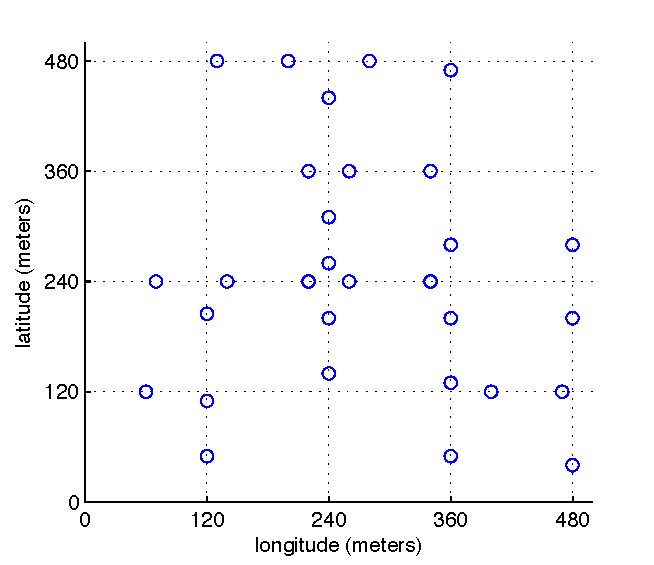
\includegraphics[width=\columnwidth]{fig/locations.pdf}
    \caption{Initial Locations of Vehicles for 30 nodes configuration}
    \label{fig:locations}
    \end{center}
    \end{figure}

    \subsubsection{Data Sharing Between Vehicle Manager and Vehicle Nodes}
    \par{We put effort in two approaches in order to enable data sharing between vehicle manager and vehicle nodes. The most naive to implement this function is to use a shared file on network file system (NFS) that all the tux hosts running vehicle nodes have access to. However, file I/O has relatively high delay, and when multiply processes are reading from and writing into the same file, there is a probability that some reading operations can fail. Thus we decided to try out a mature cache server Memcached first.}
    \begin{itemize}
    \item {\bf Memcached}
    \par{Memcached is an in-memory key-value store for small chunks of arbitrary data (strings, objects). It is widely used in industry. Web services use it as a cache layer between the web server and database for hot data. It provides APIs for data writing and retrieving.}
    \par{We designed to set up a Memcached server as a seperate process for vehicle locations data sharing. A single process, vehicle manager, was to update vehicle locations and update to Memcached server, and each vehicle node has an agent that retrieves locations from the Memcached server. Since Memcached deals with network communication and data ACID feature, the usablitiy and consistence of the data should be very reliable.}
    \par{As we use C/C++ to implement everything in our project, we used the C++ client library libmemcached to communicate with Memcached server. We implemented both vehicle manager and vehicle side agent for memcache, and we were able to validate the updating data stored in Memcached server through its concole, except that the retrieving does not work on vehicle side agent. We were not able to make the {\tt Memcache::memcache::get} work. It always complains Timeout error.}
    \par{We were not sure whether it was because we were using the API not properly or because there was a bug in libmemcached. After spending some time on it without sucess, we decided to switch to naive way, which is to use shared file on NFS.}
    \item {\bf Shared File}
    \label{sec:sharedfile}
    \par{The path to the shared file is passed through program argument. The vehicle managers keeps writing into the shared file the newest updated locations for all vehicles at a frequency of 200 milliseconds. The agent in each vehicle nodes keeps reading the shared file and update its own cache. In this way, when the sending threads need to send out messages, they can check on the cache to know which nodes are in communication range. This is pretty simple. We made it work, although, we believe it is not the best design.}
    \end{itemize}

    \subsubsection{Vehicle Manager}
    \par{As described in Section~\ref{sec:sharedfile}, the vehicle manager is in charge of simulating vehicle mobility and keeping the locations in the shared file updated. Before updating the shared file periodically, the vehicle manager needs to compute the new location for each vehicle in the map. At the very beginning, it reads in the initial locations(see Figure~\ref{fig:locations}) of all vehicles from the configuration file. Randomly speed and direction are generated for each vehicle. Each time it updates the shared file, it computes the new location based on the generated speed and the time since last time it updates the shared file. If there is any intersection between new location and old location, a left turn or right turn is possibly generated based on a probability of 0.4. Although randomly generated for each vehicle, the speed itself is mostly constant, except that we considered that the vehicle slows down when it makes turns at intersections. To simplify the model, we simply put the vehicles that decide to make turns pause at the intersection. In other words, if a vehicle needs to turn at an intersection, it stops at the intersection within this round of update no matter how much distance is left from the computation. The direction of that vehicle is then modified and in next update it will be moving.}


    \section{Testing Results}
    \par{To explore how OLSR's MPR concept can impact the EEBL broadcasting in vehicular network, we did some simple tests. We alternated our program into a second version, which does not use MPRs and simply broadcast to all vehicles within communication range. Two versions are compared on 10 - 30 vehicles with mobility. We also tested on a 30 static(without mobility) vehicles configuration in which vehicles form a connected graph.}
    \par{Figure~\ref{fig:dynamic} shows the result in dynamic traffic, in which vehicles are moving with the speed that is normally distributed with the mean of 15 m/s. It looks like the number of rebroadcasted EEBL increases exponentially. The increasing is notable from 25 nodes to 30 nodes. The MPR can greatly reduce the number of EEBL packet rebroadcasted, especially when the number of nodes is as large as 30.}
    \par{Figure~\ref{fig:static} shows the result in static configuration, in which 30 vehicles form a connected graph and do not move. In this way, two versions(with or without MPRs) are in the same situation to be compared. Again, this shows that, with MPR used, the number of EEBL rebroadcasted could be greatly rediced.}
    \begin{figure}[htb]
    \begin{center}
    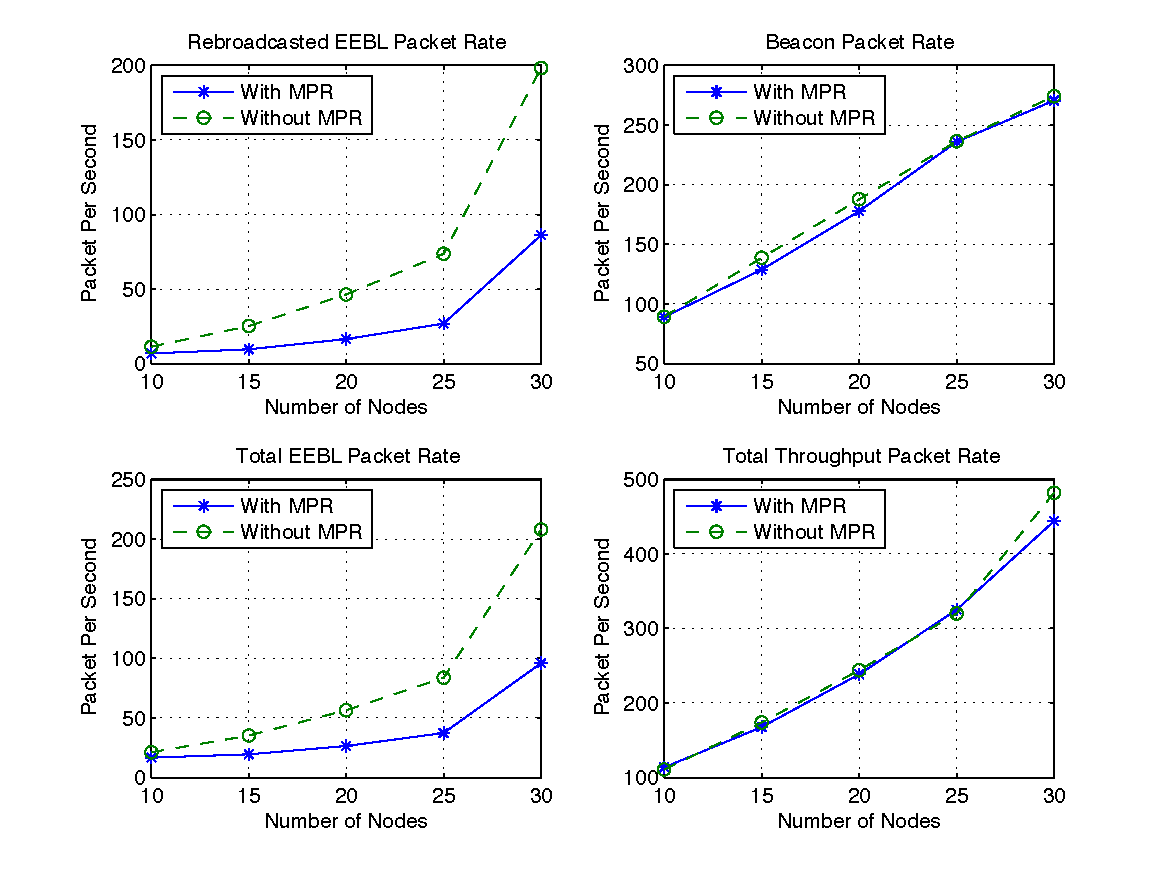
\includegraphics[width=\columnwidth]{fig/dynamic.pdf}
    \end{center}
    \par{\footnotesize{* Total EEBL = EEBL + Rebroadcasted EEBL;}}
    \par{\footnotesize{* Total Throughput = Total EEBL + Beacon + Hello Message;}}
    \caption{Packet rate for different packets for dynamic traffic}
    \label{fig:dynamic}
    \end{figure}
    \begin{figure}[htb]
    \begin{center}
    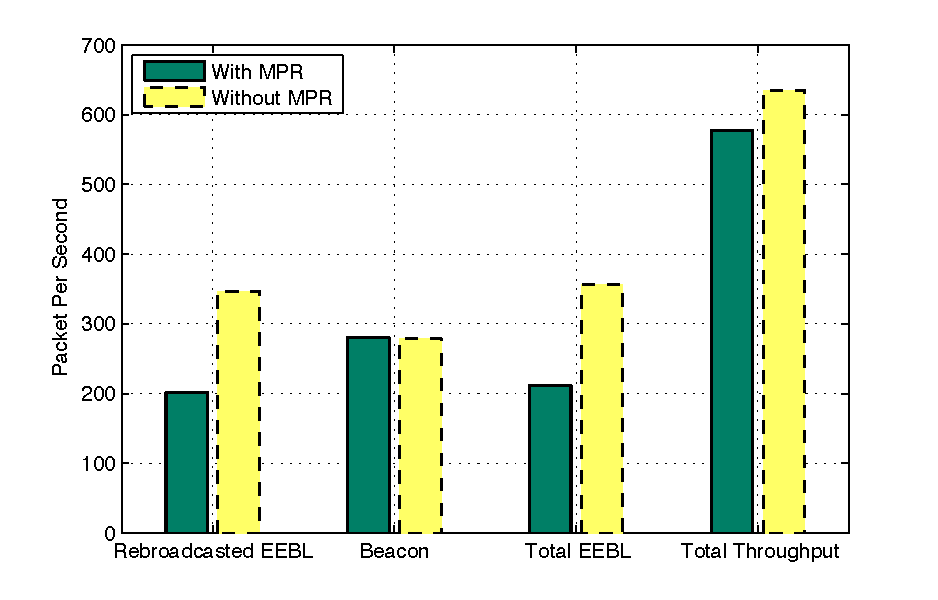
\includegraphics[width=\columnwidth]{fig/static.pdf}
    \end{center}
    \par{\footnotesize{* Total EEBL = EEBL + Rebroadcasted EEBL;}}
    \par{\footnotesize{* Total Throughput = Total EEBL + Beacon + Hello Message;}}
    \caption{Packet rate for different packets for static vehicles without mobility}
    \label{fig:static}
    \end{figure}

    \section{Conclusion}
    \par{The test results show that with OLSR's MPR concept used in EEBL rebroadcasting decision, the number of rebroadcasted messages can be greatly reduced. Since in vehicular wireless ad-hoc network, vehicles share the same wireless channel, there is channel contention among vehicles. When vehicles are close to each other, the contention becomes a serious problem and it is important to reduce the number of rebroadcasted messages. From this perspective, using MPR in rebroadcasting in vehicular network can be potentially a good approach.}
    \par{However, on the other hand, as we can see in the 'Total Throughput' part of the plots, the gap between two versions is relatively small compared to the total packet rate. As a result, the ultimate contribution to reducing network load from MPR used in vehicular network is relatively small.}



    \begin{thebibliography}{9}
    \bibitem {segata11} Michele Segata and Renato Lo Cigno. 2011. {\it Emergency braking: a study of network and application performance.} In Proceedings of the Eighth ACM international workshop on Vehicular inter-networking (VANET '11). ACM, New York, NY, USA, 1-10. DOI=10.1145/2030698.2030700 http://doi.acm.org/10.1145/2030698.2030700
    \bibitem {eeblr} O. Tonguz, N. Wisitpongphan, J. Parikh, F. Bai, P. Mudalige, and V. Sadekar. {\it On the Broadcast Storm Problem in Ad hoc Wireless Networks.} In Broadband Communications, Networks and Systems, 2006. BROADNETS 2006. 3rd International Conference on, pages 1–11, Oct. 2006.
    \bibitem {c++0xthreading} Anthony Williams. {\it Simpler Multithreading in C++0x.} \url{http://www.devx.com/SpecialReports/Article/38883/1954}
    \bibitem {memcached} Memcached Community, {\it Memcached Document.} \url{http://code.google.com/p/memcached/wiki/NewStart?tm=6}
    \end{thebibliography}
    \end{document}


